
\subsection{Feldeigenschaften des Versuchsstandes}\label{cha:4_sub_Feldeigenschaften_Versuchsstand}

Neben den geplanten Messungen zur Bestimmung der Schirmdämpfung der vorliegenden Proben sollen in diesem Abschnitt ebenfalls Messungen bezüglich einiger Feldeigenschaften innerhalb der Messkammer ausgewertet werden. Anschließend wird auf die ersten Einfügungsmessungen eingegangen und verschiedene Anpassungen vorgestellt, die zur Verbesserung der Signalqualität vorgenommen wurden. Die Gegenüberstellung der finalen Messungen mit den Werten der Vergleichsmessung erfolgt abschließend zur Validierung des Teststandes.
\par
\vspace{\linespace}
Die Befestigung des Reflektors auf dem dafür vorgesehenen Holzstativ war einer der letzten Schritte des Aufbaus. Die Wirkung auf das Übertragungsverhalten zwischen den Antennen kann anhand der folgenden \Abb\ref{fig:4_Vergleich_Reflektor} nachvollzogen werden.
\par
\vspace{\linespace}


\begin{figure}[ht]
    \centering
    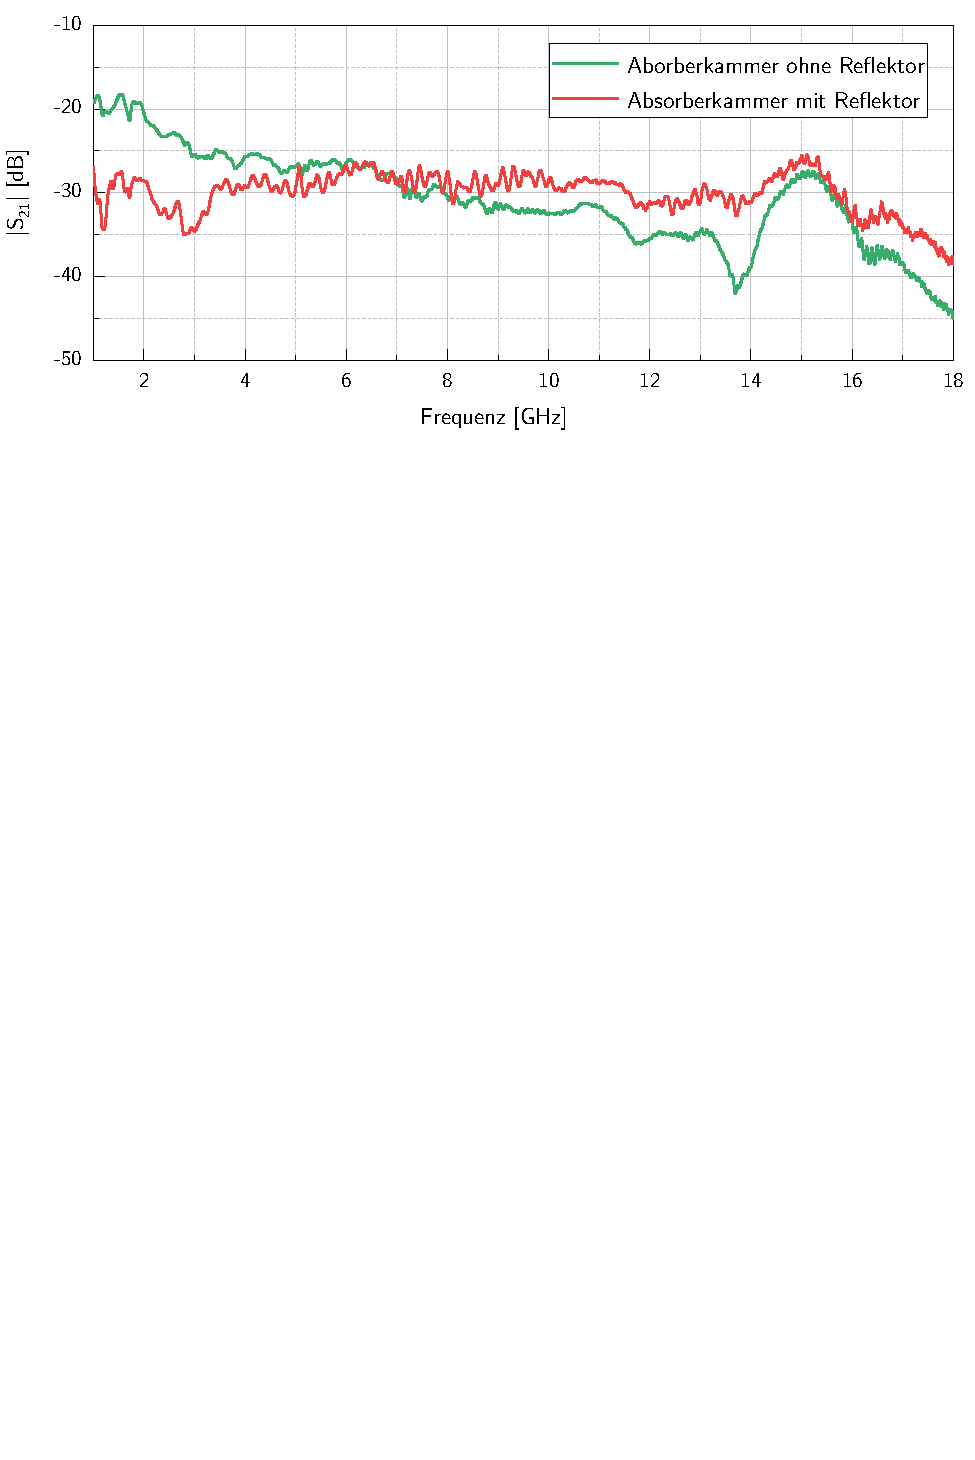
\includegraphics[page=1, width = .99\textwidth, trim = 0cm 17.3cm 0cm 0cm, clip]{Abbildungen/Kapitel4/Messergebnisse/Vergleich mit und ohne Reflektor (geerdet).pdf}
    \caption{Gemessener Transmissionskoeffizient ohne und mit eingebautem Reflektor}
    \label{fig:4_Vergleich_Reflektor}
\end{figure}

Zu erkennen ist, dass es aufgrund der Größe des Reflektorfensters vor allem im unteren Frequenzbereich zu einer erhöhten Dämpfung der Transmission kommt, was unter anderem auf die Wirkung der Öffnung als Blende zurückzuführen ist. Etwas Ähnliches kann auch beim Einfügen des Probenhalters beobachtet werden, dessen Öffnung noch kleiner ist. Die Geometrien der Öffnungen wurden, wie bereits im \Kapitel\ref{cha:3} erwähnt, unter anderem aufgrund der Größe der vorhandenen und zukünftigen Proben gewählt. Eine weitere mögliche Erklärung wäre, dass durch den Reflektor ein großer Teil der indirekten Strahlengänge über den Boden der Kammer blockiert wird, die andernfalls zu einer Verstärkung, gegenüber einer ideal absorbierenden Bodenplatte, an der Empfangsantenne führen. 
\par
\vspace{\linespace}
Die Verringerung der Freiraumdämpfung durch Einfügen des Reflektors im oberen Frequenzbereich kann wahrscheinlich auf konstruktive Interferenz mit den zusätzlich reflektierten Wellenfronten zurück\-geführt werden. Abgesehen von den auftretenden Schwankungen im Signal der Freiraum\-dämpfung mit Reflektor ist die Charakteristik und Größenordnung jedoch ebenfalls mit der Referenzmessung vergleichbar.
\par
\vspace{\linespace}
Das Einfügen des Probenhalters in die vorgesehene Halterung verändert die Charakteristik der Freiraumdämpfung nur geringfügig bis auf eine ausgezeichnete Dämpfung bei ca. \SI{1,13}{\giga\hertz} mit einem Gütefaktor

\begin{equation}
    Q = \frac{f}{B}
    %f0 = 1,1296; fL = 1,12783M; fH = 1,13151; mit -66,2252 Peaktiefe
\end{equation}

von $Q \approx 307$ (vgl. \Abb\ref{fig:4_Vergleich_Probenhalter}). Zu beachten ist hier, dass Signale unterhalb der kritischen Frequenz von $f_k \approx 1,498\;\si{\giga\hertz}$ nach \Tabelle\ref{tab:2_Grenzwellenlaengen_Hohlleiter} mit der Öffnung des Probenhalters von $a = 10\;\si{\centi\meter}$ ohnehin eine starke Dämpfung erfahren. Messungen im Bereich unter \SI{2}{\giga\hertz} sind mit dem durch die Anforderungsliste vorgegebenen Messausschnitt deshalb nur unter Vorbehalt durchzuführen. Dies wird durch die beobachtete Dämpfung bei etwas über \SI{1}{\giga\hertz} bestätigt, welche die Charakteristik der Freiraumdämpfung im Frequenzbereich zwischen \SI{0.8}{\giga\hertz} und \SI{1.6}{\giga\hertz} stark beeinflusst. %Erklärung --> Beugung oder so
\par
\vspace{\linespace}

\begin{figure}[ht]
    \centering
    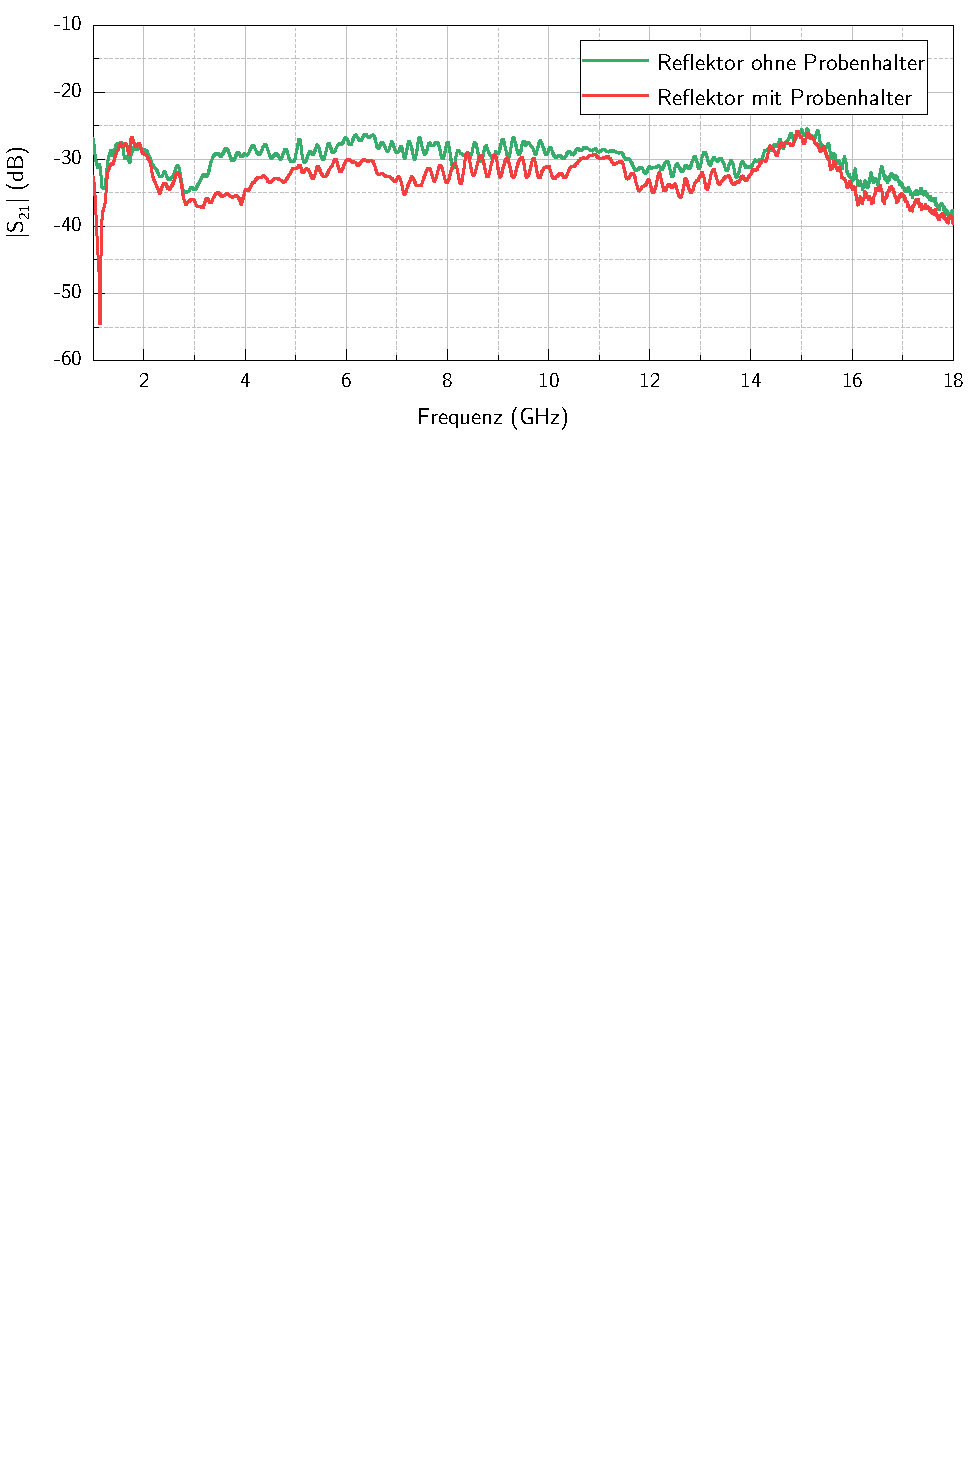
\includegraphics[page=1, width = .99\textwidth, trim = 0cm 17.3cm 0cm 0cm, clip]{Abbildungen/Kapitel4/Messergebnisse/Vergleich mit und ohne Probenhalter (geerdet).pdf}
    \caption{Gemessener Transmissionskoeffizient ohne und mit eingebautem Probenhalter}
    \label{fig:4_Vergleich_Probenhalter}
\end{figure}


Eine mögliche Erklärung, warum es aufgrund des Messausschnittes zu einem ausgezeichneten negativen Peak des gemessenen Transmissionskoeffizienten mit einem relativ hohen Gütefaktor kommt, könnte eine besonders starke Beugung der Wellen an der Öffnung des Probenhalters bei dieser spezifischen Frequenz sein. Dies würde erklären, warum eine so starke Dämpfung bei der Messung ohne Probenhalter und, wie sich im Folgenden zeigen wird, auch bei Messungen mit Proben, welche die Öffnung bis auf kleine Spalte schließen, nicht zu beobachten ist. Dies kann jedoch nur vermutet werden, da in Bezug darauf keine näheren Untersuchungen durchgeführt wurden. 
\par
\vspace{\linespace}
\newpage
Weiterhin wurde der Einfluss der Bodenplatte auf die Transmission untersucht. Dabei wurde auf Grundlage der Untersuchungen in~\cite{Vergleich_Absorberhalle_Groundplane} ein Vergleich zwischen reflektierendem Boden und einem mit Absorbern ausgelegten indirekten Koppelpfad unterhalb des Reflektors durchgeführt. Das Ziel der Betrachtung war festzustellen, inwieweit die Messungen durch die Interaktion mit vom Boden reflektierten Wellenanteilen beeinflusst werden. Die Messwerte und die Differenz beider Verläufe sind in der \Abb\ref{fig:4_Vergleich_Absorber_unter_Reflektor} dargestellt.
\par
\vspace{\linespace}

\begin{figure}[ht]
    \centering
    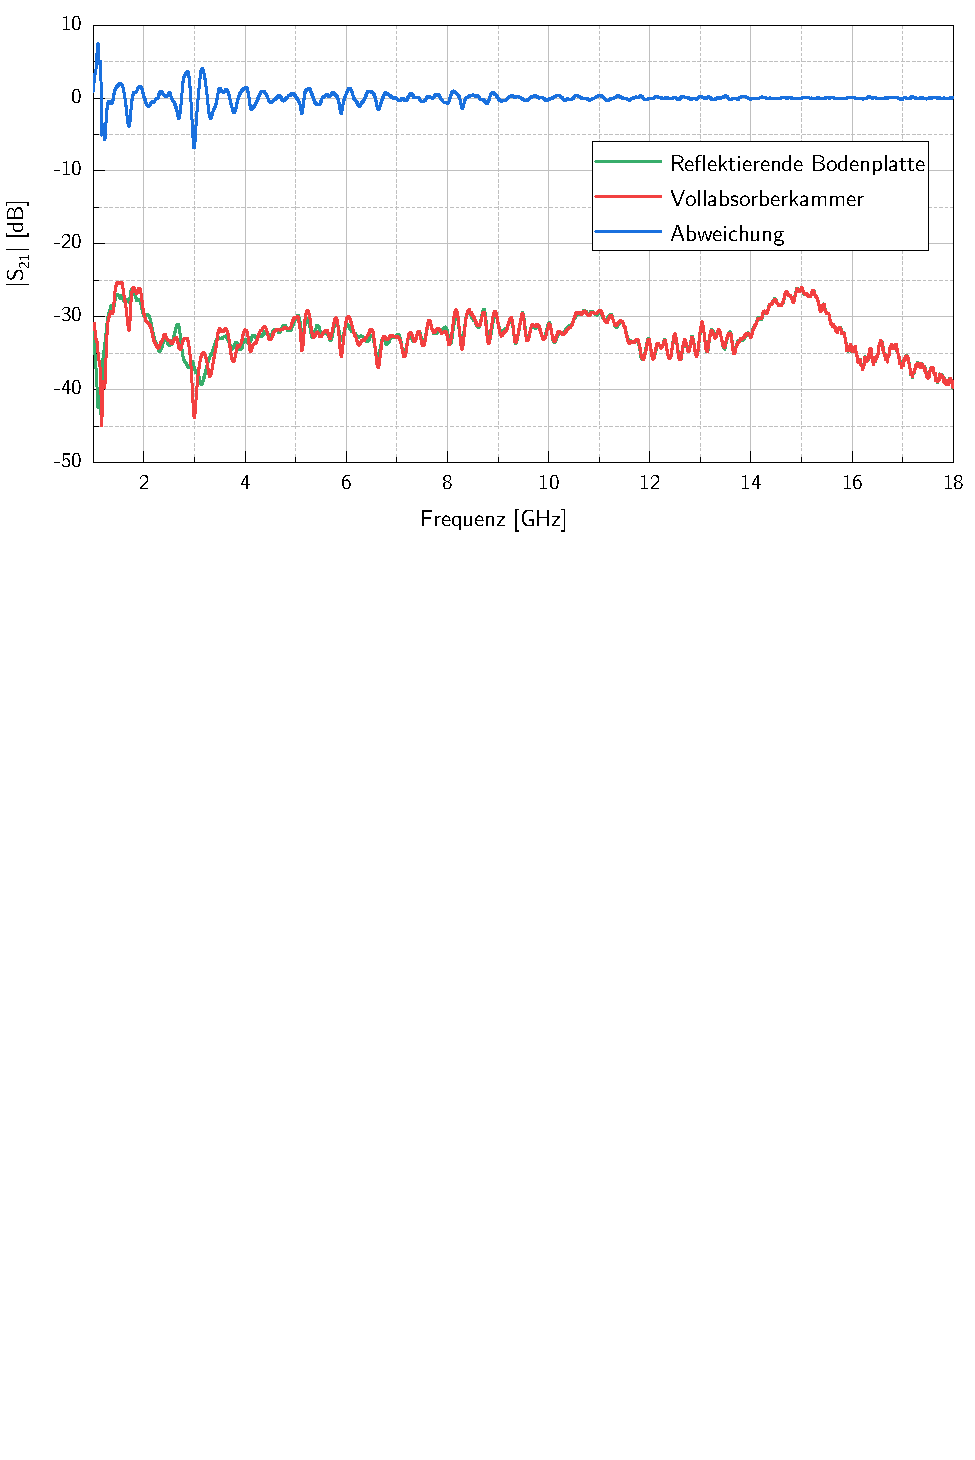
\includegraphics[page=1, width=.99\textwidth, trim = 0cm 15.6cm 0cm 0cm]{Abbildungen/Kapitel4/Messergebnisse/Vergleich Absorber unter Reflektor.pdf}
    \caption{Vergleichsmessung der Transmission mit reflektierender und absorbierender Bodenplatte}
    \label{fig:4_Vergleich_Absorber_unter_Reflektor}
\end{figure}


Zu erkennen ist, dass der Einfluss wie erwartet vor allem in den unteren Frequenzbereichen mit \mbox{Amplituden} von 5 -- \SI{10}{\Dezibel} am größten ist. Da jedoch auch oberhalb von \SI{4}{\giga\hertz} ein nicht zu vernachlässigender Einfluss zu erkennen ist, ist die Platzierung von Absorbern, vor allem direkt unterhalb des Reflektors, zur Verbesserung der Signalqualität durchaus zu empfehlen. Alle anderen Messungen wurden deshalb, wie auch im Abschnitt~\ref{cha:3_sub_Konstruktion} beschrieben, mit einer möglichst vollständig durch Absorber bedeckten Bodenplatte durchgeführt, insbesondere im Bereich der Antennenstative und unterhalb des Reflektors.
\par
\vspace{\linespace}
Da die bereits vorhandenen Stative der Antennen vollständig aus Aluminium bestehen, sollte deren Einfluss auf die Messungen ebenfalls untersucht werden. Dazu wurden die Stative sende- und empfangsseitig mit je einem Pyramidenabsorber bedeckt und eine Vergleichsmessung nur mit eingebautem Reflektor ohne Probenhalter durchgeführt. Das Ergebnis ist in \Abb\ref{fig:4_Vergleich_Absorber_vor_Stativen} ersichtlich.
\par
\vspace{\linespace}


\begin{figure}[ht]
    \centering
    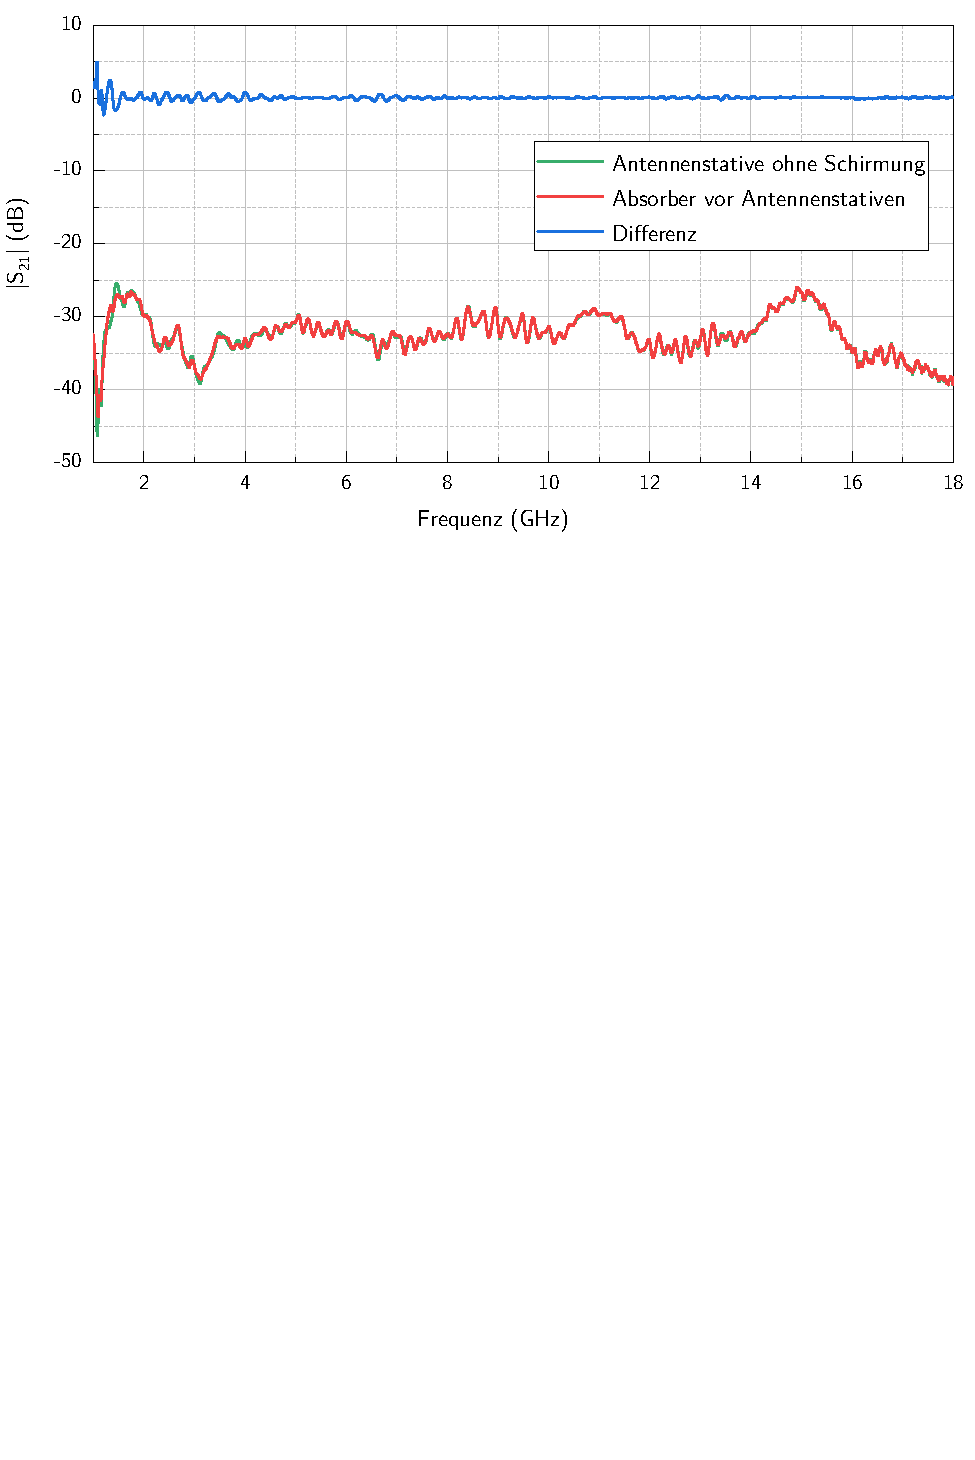
\includegraphics[page=1, width=.99\textwidth, trim = 0cm 15.6cm 0cm 0cm]{Abbildungen/Kapitel4/Messergebnisse/Vergleich Absorber vor Antennenstativen.pdf}
    \caption{Vergleichsmessung der Transmission mit unbedeckten und geschirmten Stativen}
    \label{fig:4_Vergleich_Absorber_vor_Stativen}
\end{figure}


Die zu beobachtende Differenz beider Vergleichsmessungen ist deutlich geringer als der Einfluss von platzierten Absorbern unterhalb des Reflektors und beschränkt sich im Wesentlichen auf Frequenzen unterhalb von \SI{4}{\giga\hertz}. Da die Maße der meisten stabförmigen Bestandteile der Stative die Wellenlänge des Messsignals bei \SI{4}{\giga\hertz} überschreiten, findet oberhalb dieser Frequenz kaum Beeinflussung durch als Stabantenne wirkende Teile der Stative statt. Da auch die Referenzkurven erst oberhalb von \SI{4}{\giga\hertz} beginnen, wurde die Abdeckung der Antennenstative anhand der vorliegenden Vergleichsmessung (vgl. \Abb\ref{fig:4_Vergleich_Absorber_vor_Stativen}) als eine sekundäre Maßnahme zur Verbesserung der Signalqualität gegenüber anderen eingeordnet, die im Folgenden vorgestellt werden.


\subsection{Verbesserung der Signalqualität}\label{cha:4_sub_Verbesserung_Signal}

In \Abb\ref{fig:4_erste_Messung} ist das Ergebnis der ersten mit dem Aufbau durchgeführten Schirmdämpfungsmessung dargestellt. Die Ermittlung der Schirmdämpfung aus den Messwerten der Freiraumdämpfung und der Dämpfung mit Probe wurde in \Abschnitt\ref{cha:4_Allgemeines} beschrieben. Die Bezeichnung der Probe bezieht sich auf die Balkenlänge und -breite der in die Leiterplatte eingebrachten kreuzförmigen Muster, welche in \Abb\ref{fig:4_Probenhalter_mit_Probe} zu sehen sind.
\par
\vspace{\linespace}


\begin{figure}[ht]
    \centering
    \includegraphics[page = 4, width = .99\textwidth, trim = 0cm 14.3cm 0cm 0cm, clip]{Abbildungen/Kapitel4/Messergebnisse/9k5x9k5-1.pdf}
    \caption{Erste Schirmdämpfungsmessung der Probe $9,5\times9,5-1$}
    \label{fig:4_erste_Messung}
\end{figure}


Zu erkennen ist der durch die Bearbeitung der leitfähigen Schicht der Leiterplatte hervorgerufene Bandpass im Bereich zwischen \SI{9}{\giga\hertz} und \SI{10}{\giga\hertz}. Weiterhin ist jedoch auch der Effekt der bereits beschriebenen Dämpfung bei etwas über \SI{1}{\giga\hertz} bei Messung der Freiraumdämpfung mit leerem Probenhalter zu erkennen, der sich aufgrund der Subtraktion in einer scheinbaren Verstärkung im Verlauf der Schirmdämpfung äußert. Da dieser Effekt wahrscheinlich auf die Größe des Messausschnittes zurückführbar ist, soll im Weiteren darauf nicht näher eingegangen werden. 
\par
\vspace{\linespace}
Es ist außerdem ersichtlich, dass die ermittelte Schirmdämpfung im Bereich des Bandpasses und vor allem bei hohen Frequenzen teilweise stark fluktuiert. Um die Ursache hierfür zu ermitteln und die Qualität der Messung zusätzlich zu verbessern, wurden die nachfolgenden Anpassungen, deren Ergebnisse in den \Abbildungen\ref{fig:4_9k5x9k5-1_Erdung} --~\ref{fig:4_9k5x9k5-1_Schrauben} ersichtlich sind, vorgenommen. Anzumerken ist, dass alle abgebildeten Messsignale stabil waren und sich auch über mehrere Scandurchläufe, abgesehen vom zufälligen Rauschen, nicht veränderten. Weiterhin wurden alle Konnektoren bezüglich einer korrekten Verschraubung überprüft, sodass dies als Ursache für die Fluktuationen auszuschließen ist. Die Kalibration des VNA wurde ebenfalls wie in \Abschnitt\ref{cha:4_Kalibration_Messtechnik} beschrieben durchgeführt. 
\par
\vspace{\linespace}
Die zusätzliche Erdung des Reflektors durch Verbindung mit der geerdeten äußeren Schirmhülle der Testkammer hat einen positiven Einfluss über dem gesamten Frequenzbereich (vgl. \Abb\ref{fig:4_9k5x9k5-1_Erdung}). Entsprechend der durchgeführten Versuche war dabei die Verbindung mit der Wand des Messkabine ausreichend für die Verbesserung, auch wenn letztere nicht mit dem Erdpotenzial verbunden war.  
\par
\vspace{\linespace}

\begin{figure}[H]
    \centering
    \includegraphics[page = 2, width = .99\textwidth, trim = 0cm 16.8cm 0cm 0cm, clip]{Abbildungen/Kapitel4/Messergebnisse/9k5x9k5-1.pdf}
    \caption[Vergleich des Einflusses der Erdung auf die Messwerte]{Vergleich des Einflusses der Erdung auf die Messwerte für \mbox{$9,5\times9,5-1$}}
    \label{fig:4_9k5x9k5-1_Erdung}
\end{figure}

\newpage

Die Platzierung zusätzlicher Absorber neben der Öffnung des Reflektors hat bis auf kleine Bereiche keinen nennenswerten Einfluss auf die zu beobachtenden Fluktuationen des Signals (vgl. \Abb\ref{fig:4_9k5x9k5-1_Absorberplatzierung}). Dies ist wahrscheinlich darauf zurückzuführen, dass Wellenanteile, welche an dieser Stelle auf den Reflektor treffen, aufgrund des Winkels, in dem sie reflektiert werden, das Messsignal auch ohne zusätzliche Dämpfung nicht beeinflussen und zu großen Teilen auf die Absorber an den Wänden treffen.
\par
\vspace{\linespace}
Im Gegensatz dazu kann insbesondere im Bereich des Bandpasses zwischen \SI{8}{\giga\hertz} und  \SI{11}{\giga\hertz} eine deutliche Verbesserung durch Platzierung von Absorberstreifen über den Befestigungsschrauben und -muttern des Probenhalters erzielt werden. Da die Abmessungen der damit abgedeckten Befestigungselemente etwa in der Größenordnung der halben Wellenlänge des erwähnten Frequenzbereiches liegen, ist die Beeinflussung des Signals hier wahrscheinlich darauf zurückzuführen. 
\par
\vspace{\linespace}

\begin{figure}[ht]
    \centering
    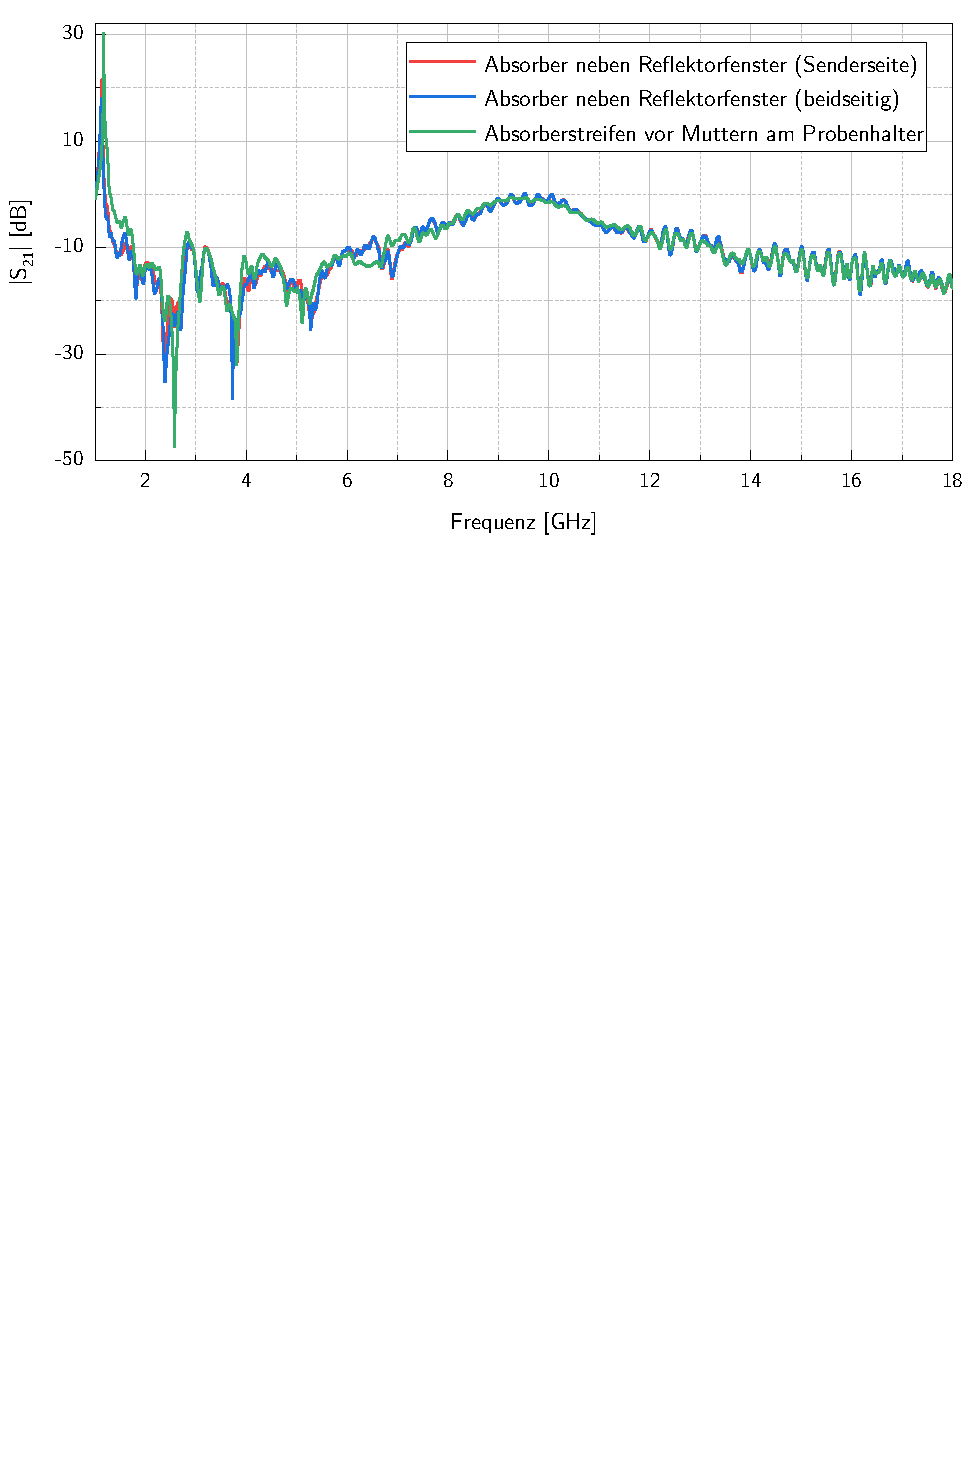
\includegraphics[page = 1, width = .99\textwidth, trim = 0cm 16.8cm 0cm 0cm, clip]{Abbildungen/Kapitel4/Messergebnisse/9k5x9k5-1.pdf}
    \caption[Vergleich des Einflusses der Platzierung zusätzlicher Absorber auf die Messwerte]{Vergleich des Einflusses der Platzierung zusätzlicher Absorber auf die Messwerte für \mbox{$9,5\times9,5-1$}}
    \label{fig:4_9k5x9k5-1_Absorberplatzierung}
\end{figure}

Auf Basis dieses Ergebnisses wurde weiterhin untersucht, ob sich eine Verbesserung ebenfalls durch Austauschen der verwendeten Flügelmuttern zum Verschrauben des Probenhalters durch Sechskantmuttern, sowie durch reines Verklemmen beider Hälften des Probenhalters erzielen lässt (vgl. \Abb\ref{fig:4_9k5x9k5-1_Schrauben}). Auch dabei konnte keine nennenswerte Reduktion der Signalfluktuation beobachtet werden. Abschließend wurde getestet, ob sich durch Verwendung von Abstandshaltern zwischen den Hälften des Probenhalters, die den gleichen Abstand herstellen, wie er auch bei der Messung mit den Leiterplatten vorhanden ist, eine Verbesserung der Signalqualität erreichen lässt. Wie die \Abb\ref{fig:4_9k5x9k5-1_Schrauben} zeigt, ist dies ebenfalls im Bereich des Bandpasses der Fall und die Amplitude der verbleibenden Fluktuation ist mit der zu vergleichen, die durch Platzierung von Absorberstreifen über den Schrauben und Muttern erreicht wurde. 
\par
\vspace{\linespace}

\begin{figure}[ht]
    \centering
    \includegraphics[page = 3, width = .99\textwidth, trim = 0cm 16.8cm 0cm 0cm, clip]{Abbildungen/Kapitel4/Messergebnisse/9k5x9k5-1.pdf}
    \caption[Vergleich des Einflusses der Schrauben des Probenhalters auf die Messwerte]{Vergleich des Einflusses der Schrauben des Probenhalters auf die Messwerte für \mbox{$9,5\times9,5-1$}}
    \label{fig:4_9k5x9k5-1_Schrauben}
\end{figure}


Zusätzlich konnte die Fluktuation oberhalb von \SI{12}{\giga\hertz} durch Abkleben der Schnittkanten des Reflektorfensters mit Aluminiumklebeband weiter reduziert werden. Eine verbleibende Ursache für das stark zerrissene Signal im oberen Messbereich könnte die verstärkte Reflektion durch Schließen des Reflektorfensters mit der zu messenden Probe sein. Diese wirkt oberhalb des Bandpasses ebenfalls reflektierend. In \Abb\ref{fig:4_finaler_Aufbau} ist die Senderseite der finalen Konfiguration dargestellt.

\begin{figure}[H]
    \centering
    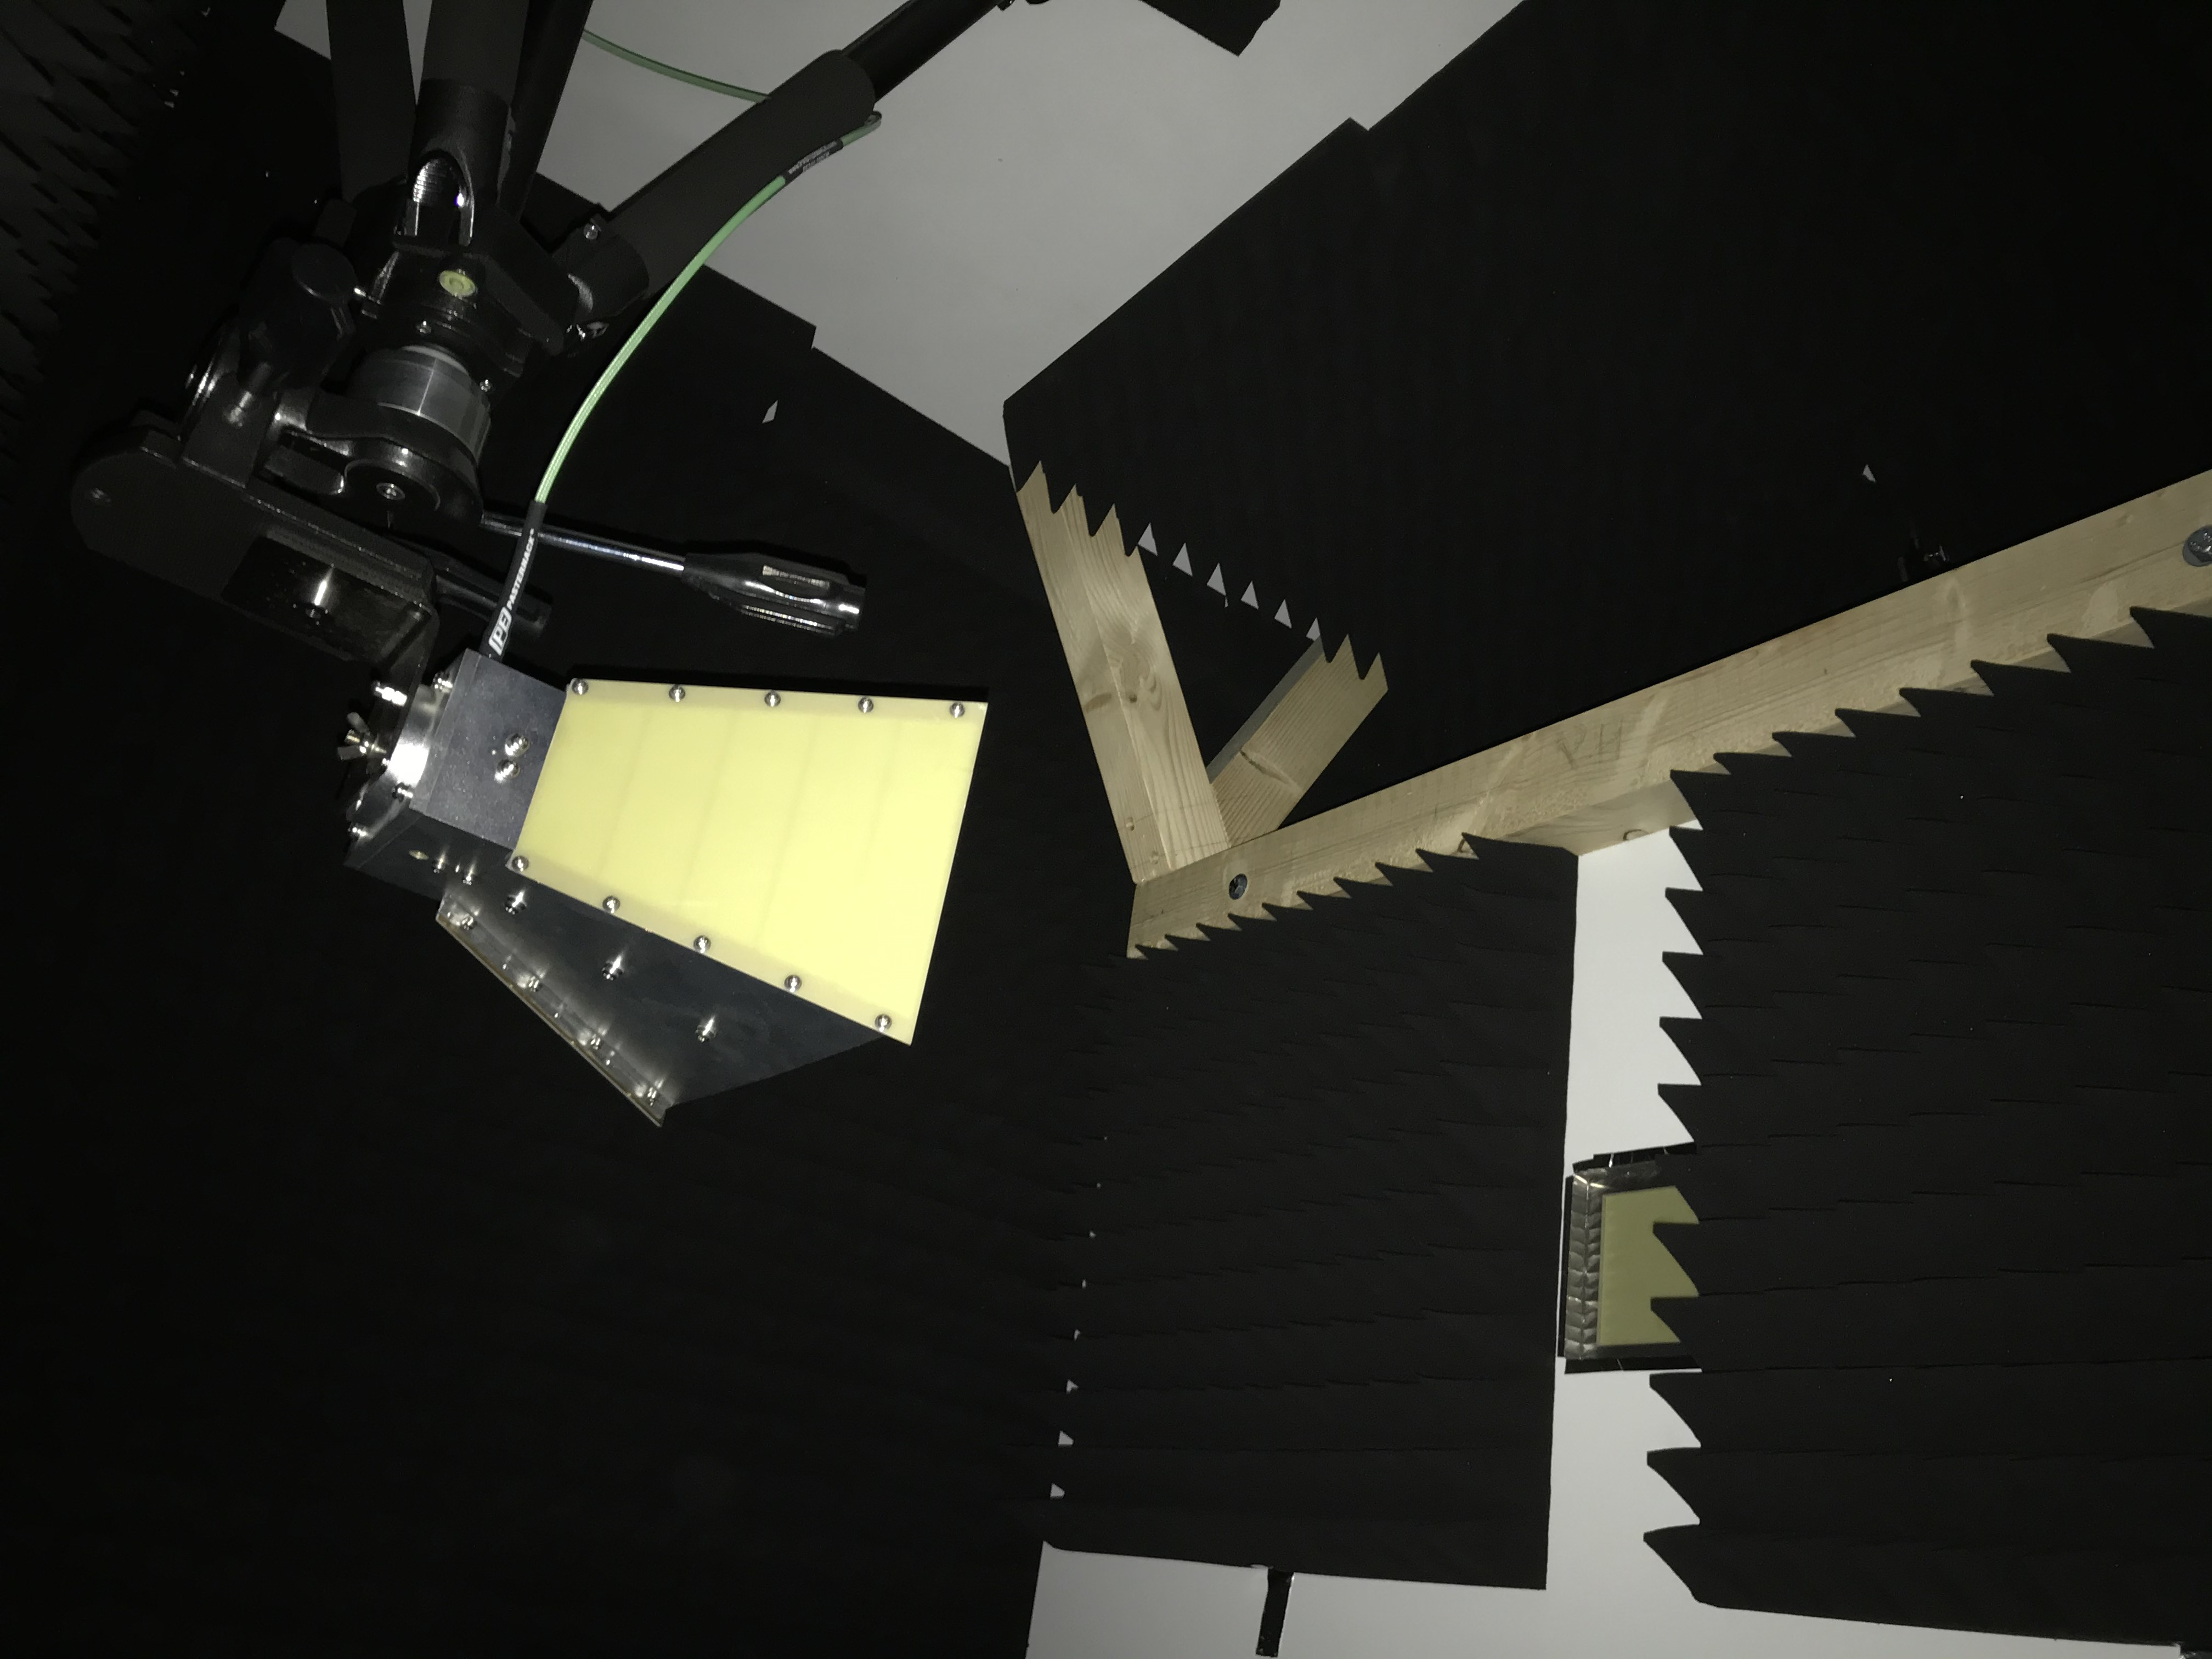
\includegraphics[height=.25\textheight, draft = false]{Abbildungen/Kapitel4/IMG_5719.jpg}
    \caption{Senderseitige Messstrecke mit finaler Absorberplatzierung und abgeklebtem Reflektorfenster}
    \label{fig:4_finaler_Aufbau}
\end{figure}


\subsection{Analyse der Messwerte und Vergleich mit Referenzmessungen}\label{cha:4_sub_Analyse_und_Vergleich}

In der \Abb\ref{fig:4_Messwerte} sind die unter Anwendung der vorgestellten Anpassungen ermittelten Messwerte der Transmissionskoeffizienten aller untersuchten Proben zusammengefasst. Da hier zusätzlich zu den Dämpfungswerten der Leiterplatten ebenfalls ein Aluminiumblech und Buckypaper, ein Aggregat aus \acp{CNT}, vermessen wurden, kann auf die Ursache weiterer Charakteristika in den Dämpfungskurven geschlossen werden. Im Gegensatz zu den Leiterplatten besitzt beispielsweise ein \SI{0,5}{\milli\meter} starkes Aluminiumblech für Wellenfelder zwischen \SI{1}{\giga\hertz} und \SI{18}{\giga\hertz} eine theoretische Dämpfung von mehr als \SI{100}{\Dezibel}~\cite{EM_Schirmung}. Damit lässt sich feststellen, ob der Probenhalter bzw. der Durchgang durch das Reflektorfenster einen Einfluss auf den Verlauf in bestimmten Frequenzbereichen hat. Aufgrund der sehr hohen Schirmdämpfung sollten bei der Messung mit der Aluminiumplatte diese Charakteristika, die beim Durchgang durch die Probenhalterung verursacht werden, nicht zu beobachten sein.
\par
\vspace{\linespace}

\begin{figure}[ht]
    \centering
    \includegraphics[page = 1, width = .99\textwidth, trim = 0cm 13cm 0cm 0cm, clip]{Abbildungen/Kapitel4/Messergebnisse/Messwerte.pdf}
    \caption{Transmissionskoeffizienten der vermessenen Probetypen}
    \label{fig:4_Messwerte}
\end{figure}

Die im Bereich von \SI{2}{\giga\hertz} bis \SI{3,5}{\giga\hertz} auftretenden Minima sind bei allen Kurven außer der Freiraumdämpfung zu erkennen, sodass die Vermutung nahe liegt, dass es sich hierbei um Interferenzen mit an den Proben reflektierten Wellenanteilen handelt, da auch die Leiterplatten in diesem Frequenzbereich eine hohe Dämpfung aufweisen. Die nachfolgenden drei ausgezeichneten Extremstellen zwischen \SI{3,5}{\giga\hertz} und \SI{7}{\giga\hertz} treten nur bei den frequenzselektiven Proben auf. Ein ähnlicher Verlauf kann auch bei den Referenzmessungen beobachtet werden~\cite{FSS_Toedter_Diplomarbeit}. Da die Messungen mit Aluminium und Buckypaper diesen Verlauf nicht zeigen, kann angenommen werden, dass diese Minima dadurch entstehen, dass Wellenanteile durch die frequenzselektiven Schichten dringen und mit Teilen der Probenhalterung interagieren. Zu beachten ist, dass dieser Verlauf bei der gemessenen Freiraumdämpfung nicht auftritt und damit nicht allein auf die Probenhalterung zurückzuführen ist. 
\par
\vspace{\linespace}
Die oberhalb von \SI{10}{\giga\hertz} erkennbare Charakteristik der Freiraumdämpfung ist ebenfalls in den \mbox{Kurven} aller Leiterplatten zu erkennen. Somit ist die Beeinflussung durch das Reflektorfenster und den Probenhalter hier als Hauptursache anzunehmen.
\par
\vspace{\linespace}
Weiterhin liegt die gemessene Schirmdämpfung der Aluminiumplatte und des Buckypaper weit unterhalb der theoretischen, anhand der hohen Leitfähigkeit beider Materialien zu erwartenden, Einfügungsdämpfung. Der Verlauf beider Messkurven ähnelt außerdem der Reflektionsdämpfung der verwendeten Pyramidenabsorber~\cite{Eco_Messtechnik_Absorber}. Es ist davon auszugehen, dass hier die maximal messbare Einfügungsdämpfung durch die Reflektionsdämpfung der Absorber, welche seitlich um den Reflektor angeordnet sind, begrenzt ist. Das Messsignal besteht demnach aus Wellen, die über den indirekten Koppelpfad trotz der vorhandenen Absorber zur Empfangsantenne gelangen. Das Befestigungskonzept der Probenhalterung scheint somit für den vorliegenden Aufbau geeignet, da bei vollständigem Abschluss der Öffnung so gut wie keine Wellenanteile durch die Halterung zu dringen scheinen und gemessen werden.
\par
\vspace{\linespace}





%zwischen 2 und 4 GHz gleicher Verlauf bei allen Proben --> scheint Eigenschaft der Kammer selbst bzw. der Absorber zu sein
%zwische 4 und 6 nur Dipps bei Leiterplatten zu erkennen, die dort einen Teil der Welle durchlassen --> scheint Eigenschaft des Probenhalters zu sein
%Auch Charakteristik im hinteren Bereich (Buckel bei 15GHz) scheint auf PH zurückführbar, weil bei anderen Proben nicht auftritt, bei denen theoretisch keine Leistung durch das Reflektorfenster dringt



Die nachfolgenden \Abbildungen\ref{fig:4_Schirmdämpfung_9k5x9k5-1} bis~\ref{fig:4_Schirmdämpfung_10k5x10k5-1} zeigen die aus den obigen Rohdaten ermittelten Schirmdämpfungen für die frequenzselektiven Proben. Um die auftretenden Schwankungen des Messsignals zur besseren Auswertung der vorhandenen Bandpässe weiter zu reduzieren, wurde auf alle Kurven ein Savitzky-Golay-Filter angewandt. Es handelt sich dabei um einen gleitenden Signalfilter, welcher eine polynomiale Regression über einer Serie von Stützpunkten liefert~\cite{Savitzky-Golay-Filter_Original}. Je nach Anpassung der verwendeten Koeffizienten kann diese Methode auch als gleitende Mittelwertsbildung wirken. Der Vorteil dieser Filterung ist, dass sie die Charakteristik des Signals und auch Anteile hoher Frequenzen erhält~\cite{Savitzky-Golay-Filter_Original}. Im Auswertungsprogramm für Schirmdämpfungsmessungen, welches im digitalen Anhang auf der CD enthalten ist, ist die Filterung nach Savitzky-Golay als Option verfügbar und kann durch Einstellung des Polynomgrades und Anzahl der verwendeten Stützstellen für die Regression angepasst werden.
\par
\vspace{\linespace}
Im direkten Vergleich der Verläufe ist zu erkennen, dass auch die Referenzmessungen eine mäandernde Charakteristik mit Extremstellen in etwa den gleichen Frequenzbereichen aufweisen. Da dort die gleichen Proben und ein ähnlicher Messaufbau, wenn auch mit vollständiger Trennung von Sende- und Empfangsbereich, genutzt wurden~\cite{FSS_Toedter_Diplomarbeit}, lässt dies den Schluss zu, dass diese Merkmale inhärente Eigenschaften der Schirmdämpfungsmessung unter Realbedingungen sind. Außerdem war anhand der Messwerte festzustellen, dass die im \Abschnitt\ref{cha:4_Allgemeines} beschriebene Reziprozität für den Aufbau mit \mbox{$|S_{12}| \approx |S_{21}|$ gilt}.
\par
\vspace{\linespace}

\begin{figure}[H]
    \centering
    \includegraphics[page=3, width=.99\textwidth, trim = 0cm 14.3cm 0cm 0cm, clip]{Abbildungen/Kapitel4/Messergebnisse/Messwerte.pdf}
    \caption{Schirmdämpfung und gefilterter Verlauf für $9,5\times9,5-1$}
    \label{fig:4_Schirmdämpfung_9k5x9k5-1}
\end{figure}

\begin{figure}[H]
    \centering
    \includegraphics[page=4, width=.99\textwidth, trim = 0cm 14.3cm 0cm 0cm, clip]{Abbildungen/Kapitel4/Messergebnisse/Messwerte.pdf}
    \caption{Schirmdämpfung und gefilterter Verlauf für $10\times10-0,5$}
    \label{fig:4_Schirmdämpfung_10x10-0k5}
\end{figure}

\begin{figure}[H]
    \centering
    \includegraphics[page=2, width=.99\textwidth, trim = 0cm 14.3cm 0cm 0cm, clip]{Abbildungen/Kapitel4/Messergebnisse/Messwerte.pdf}
    \caption{Schirmdämpfung und gefilterter Verlauf für $10\times10-1$}
    \label{fig:4_Schirmdämpfung_10x10-1}
\end{figure}

\begin{figure}[H]
    \centering
    \includegraphics[page=5, width=.99\textwidth, trim = 0cm 14.3cm 0cm 0cm, clip]{Abbildungen/Kapitel4/Messergebnisse/Messwerte.pdf}
    \caption{Schirmdämpfung und gefilterter Verlauf für $10\times10-1,5$}
    \label{fig:4_Schirmdämpfung_10x10-1k5}
\end{figure}

\begin{figure}[H]
    \centering
    \includegraphics[page=6, width=.99\textwidth, trim = 0cm 14.3cm 0cm 0cm, clip]{Abbildungen/Kapitel4/Messergebnisse/Messwerte.pdf}
    \caption{Schirmdämpfung und gefilterter Verlauf für $10,5\times10,5-1$}
    \label{fig:4_Schirmdämpfung_10k5x10k5-1}
\end{figure}

\newpage

Wichtiger für die Charakterisierung der frequenzselektiven Proben sind jedoch die Bandpässe, d.h. die Stellen der minimalen Schirmdämpfung und die zugehörige Bandbreite. Nach den Ausführungen in \Abschnitt\ref{cha:4_sub_Feldeigenschaften_Versuchsstand} wurde hierfür die Überhöhung bei ca. \SI{1.13}{\giga\hertz} nicht einbezogen, da diese auf den Versuchsstand zurückzuführen ist. Die Tabelle~\ref{tab:4_Messwerte} fasst die aus den Messwerten ermittelten Ergebnisse zusammen. 
\par
\vspace{\linespace}

\begin{table}[ht]
    \centering
    \renewcommand{\arraystretch}{1.2}
    \caption{Zusammenfassung der Messergebnisse für die Bandpässe der frequenzselektiven Proben}\label{tab:4_Messwerte}
    \vspace{\tablespace}
    \begin{tabular}{p{2.5cm} R{1cm} R{1cm} R{1cm} R{1cm} p{0.25cm} R{1cm} R{1cm} R{1cm} R{1cm}}
        \toprule
        \multirow[b]{2}{*}{\textbf{Probe}} & \multicolumn{4}{c}{\textbf{Werte für Rohdaten [GHz]}} && \multicolumn{4}{c}{\textbf{Werte für gefiltertes Signal [GHz]}} \\
          & \multicolumn{1}{c}{{\boldmath$f_0$}} & \multicolumn{1}{c}{{\boldmath$f_L$}} & \multicolumn{1}{c}{{\boldmath$f_H$}} & \multicolumn{1}{c}{\textbf{BW}} && \multicolumn{1}{c}{{\boldmath$f_0$}} & \multicolumn{1}{c}{{\boldmath$f_L$}} & \multicolumn{1}{c}{{\boldmath$f_H$}} & \multicolumn{1}{c}{\textbf{BW}} \\
        \midrule
        $9,5\times9,5-1$   & 9,53 & 8,65 & 10,61 & 1,97 && 9,44 & 8,53 & 10,65 & 2,12 \\
        $10\times10-0,5$   & 9,00 & 8,31 & 9,58 & 1,28  && 8,96 & 8,30 & 9,48 & 1,18 \\
        $10\times10-1$     & 9,02 & 7,80 & 9,93 & 2,13  && 9.02 & 7,84 & 10,16 & 2,32 \\
        $10\times10-1,5$   & 9,02 & 7,78 & 10,44 & 2,66 && 9,02 & 7,59 & 10,47 & 2,88 \\
        $10,5\times10,5-1$ & 7,94 & 7,25 & 9,06 & 1,82  && 7,97 & 7,15 & 9,33 & 2,18 \\
        \bottomrule
    \end{tabular}
    \vspace*{\linespace}
\end{table}

Die in~\cite{FSS_Toedter_Diplomarbeit} gefundenen Zusammenhänge zwischen der Balkenlänge der in die Leitschicht eingebrachten Kreuzmuster (vgl. \Abb\ref{fig:4_Probenhalter_mit_Probe}) und der 3dB-Bandbreite (BW) sowie der Balkendicke und der Verschiebung der Extremstelle kann anhand dessen bestätigt werden.
\par
\vspace{\linespace}
Die ermittelten Ergebnisse (vgl. \Tabelle\ref{tab:4_Messwerte}) weisen insgesamt nur geringe Abweichungen zu den Werten der Vergleichsmessung auf. Anzumerken ist, dass die Grundfrequenz der Bandpässe, bei der die erreichte Schirmdämpfung gegen \SI{0}{\Dezibel} geht, aus den Rohdaten zum Teil genauer bestimmt werden konnte, als bei Verwendung der gefilterten Signale. Die Genauigkeit ist dabei bezogen auf die Abweichung zur Referenzmessung. Die gefilterten Verläufe lieferten jedoch teilweise Werte mit einer geringeren Abweichung für die untere und obere Grenzfrequenz der Bandbreite. In der \Tabelle\ref{tab:4_Abweichungen_Messwerte} sind die Abweichungen aller Ergebnisse aufgetragen. 
\par
\vspace{\linespace}

\begin{table}[ht]
    \centering
    \renewcommand{\arraystretch}{1.3}
    \caption[Abweichung der Messergebnisse von den Vergleichswerten der Referenzmessung]{Abweichungen der Messergebnisse von den Vergleichswerten der Referenzmessung~\cite{FSS_Toedter_Diplomarbeit}}
    \label{tab:4_Abweichungen_Messwerte}
    \vspace{\tablespace}
    \begin{tabular}{p{2.5cm} R{1.1cm} R{1.1cm} R{1.1cm} R{1.2cm} p{0.25cm} R{1.1cm} R{1.1cm} R{1.1cm} R{1.2cm}}
        \toprule
        \multirow[b]{2}{*}{\textbf{Probe}} & \multicolumn{4}{c}{\textbf{Abweichung für Rohdaten}} && \multicolumn{4}{c}{\textbf{Abweichung für gefiltertes Signal}} \\
          & \multicolumn{1}{c}{{\boldmath$f_0$}} & \multicolumn{1}{c}{{\boldmath$f_L$}} & \multicolumn{1}{c}{{\boldmath$f_H$}} & \multicolumn{1}{c}{\textbf{BW}} && \multicolumn{1}{c}{{\boldmath$f_0$}} & \multicolumn{1}{c}{{\boldmath$f_L$}} & \multicolumn{1}{c}{{\boldmath$f_H$}} & \multicolumn{1}{c}{\textbf{BW}} \\
        \midrule
        $9,5\times9,5-1$   & 1,14\% & 2,22\% & 1,87\% & 0,34\% && 0,21\% & 0,81\% & 2,17\% & 8,04\% \\
        $10\times10-0,5$   & 0,01\% & 2,29\% & 0,40\% & 14,93\% && 0,47\% & 2,17\% & 1,46\% & 21,09\% \\
        $10\times10-1$     & 0,04\% & 0,20\% & 0,28\% & 0,55\% && 0,05\% & 0,27\% & 2,04\% & 8,49\% \\
        $10\times10-1,5$   & 0,26\% & 1,82\% & 0,53\% & 3,05\% && 0,25\% & 0,63\% & 0,86\% & 5,01\% \\
        $10,5\times10,5-1$ & 0,73\% & 0,57\% & 1,37\% & 13,53\% && 0,36\% & 1,89\% & 0,64\% & 3,72\% \\
        \bottomrule
    \end{tabular}
\end{table}

Die bestehenden Zusammenhänge zwischen den Veränderungen der frequenzselektiven Oberflächen und dem Einfluss auf den Bandpass können grafisch ebenfalls sehr gut nachvollzogen werden. Die \Abbildungen\ref{fig:4_Variation_Balkenlaenge} und~\ref{fig:4_Variation_Balkenbreite} verdeutlichen dies im direkten Vergleich zu den Ergebnissen aus~\cite{FSS_Toedter_Diplomarbeit}.
\par
\vspace{\linespace}


\begin{figure}[H]
    \centering
        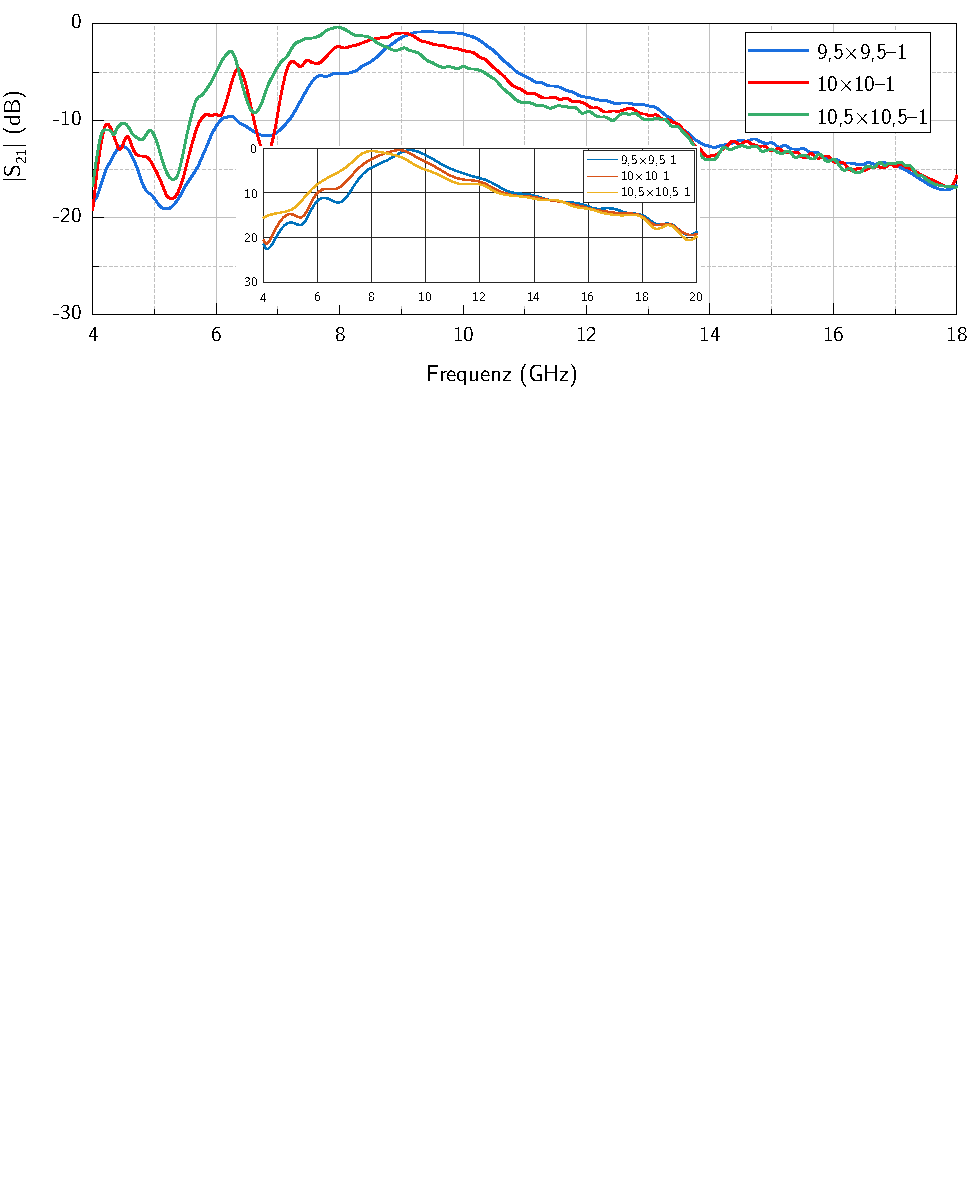
\includegraphics[page=1, width=.99\textwidth, trim = 0cm 13.3cm 0cm 0cm, clip]{Abbildungen/Kapitel4/Messergebnisse/Vergleich_Balkenlaenge.pdf}
    \caption[Veränderung des Bandpasses durch Variation der Balkenlänge]{Veränderung des Bandpasses durch Variation der Balkenlänge und Vergleichsplots~\cite{FSS_Toedter_Diplomarbeit}}\label{fig:4_Variation_Balkenlaenge}
\end{figure}

\begin{figure}[H]
    \centering
    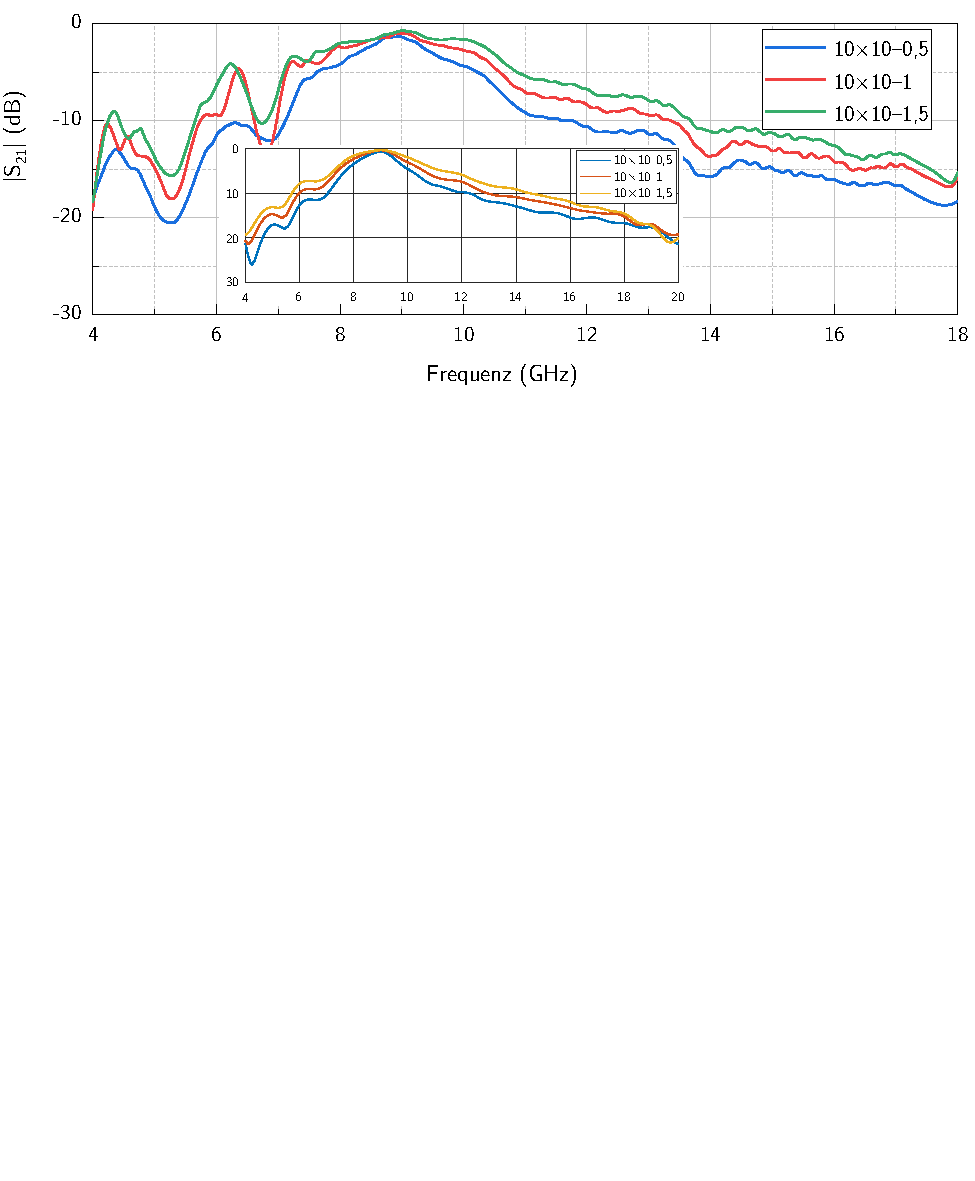
\includegraphics[page=1, width=.99\textwidth, trim = 0cm 13.3cm 0cm 0cm, clip]{Abbildungen/Kapitel4/Messergebnisse/Vergleich_10x10.pdf}
    \caption[Veränderung des Bandpasses durch Variation der Balkenbreite]{Veränderung des Bandpasses durch Variation der Balkenbreite und Vergleichsplots~\cite{FSS_Toedter_Diplomarbeit}}\label{fig:4_Variation_Balkenbreite}
\end{figure}


Wie bereits erwähnt unterschieden sich die Messdaten zweier aufeinanderfolgender Scandurchläufe nur durch das statistische Rauschen. Weiterhin konnte auch bei Messungen der gleichen Probe an unterschiedlichen Tagen kein Unterschied festgestellt werden, der die Genauigkeit der ermittelten Charakteristiken der Bandpässe oder die Verläufe der Schirmdämpfungen signifikant beeinflusst. Somit ist die durch den konstruktiven Entwicklungsprozess angestrebte Wiederholbarkeit von Messungen gewährleistet. 
\par
\vspace{\linespace}
Weiterhin können anhand der durchgeführten Versuche die Messergebnisse in~\cite{FSS_Toedter_Diplomarbeit} bestätigt werden. Die Funktionsweise des Messstandes für Schirmdämpfungsmessungen wurde durch Vergleich der Ergebnis\-größen und der gemessenen Verläufe der Einfügungsdämpfung über dem Messbereich nachgewiesen. Die Eigenschaften der vorhandenen Bandpässe der frequenzselektiven Proben konnten mit einer sehr geringen Abweichung ermittelt werden. Der Versuchsstand ist damit entsprechend den Anforderungen für die Messung der Schirmdämpfung unterschiedlicher Probetypen im Fernfeld validiert. 




%kein Unterschied feststellbar bei zwei Messungen ohne Probe an unterschiedlichen Tagen, da etwas gleiche Bedingungen und keine Veränderungen an Signalkabeln, etc zwischen Messungen nach Kalibration


%Ohne Erdung verstärkt sich Rauschen leicht, vor allem im hohen Frequenzbereich; kaum Unterschieschied, ob nur mit Schirm verbunden oder auch geerdet

%Absorber vor Antennen hat vor allem Auswirkungen im unteren Frequenzbereich
%gleiches gilt für Absorber unter Reflektor zur Reduktion von sekundären Wellenfronten --> Aussage aus \cite bestätigt, kein Einfluss ab ..GHz feststellbar

%Abkleben der Schnittkante des Reflektors hat weiterhin Einfluss, vor allem im hohen Frequenzbereich

%Peak aufgrund von Cut-Off und Beugungserscheinungen --> je besser Rest der Kurve aussieht, desto steiler wird Peak --> letztendlich bei 1,12965 GHz = 26,5385 cm Wellenlänge



%--> Schirmdämpfungsplots mit verschiedenen Anpassungen in ein Diagramm
        %-erste Messung, keine Anpassung
        %-Erdung
        %-normale Schrauben
        %-Absorber an Reflektor (hinten)
        %-Absorber an Reflektor (beidseitig)
        %-normale Schrauben und Abstand bei Messung ohne Probe
        %-keine Schrauben
        %-Absorber an PH



%An allen Varianten kann wie vermutet festgestellt werden, dass Reziprozität gilt, d.h. Werte für S12 und S21 sind bis auf das statistische Rauschen gleicht




%Erklärung für zerrissenes Signal: Reflektionen, die schon bei PLatzioerung des Reflektors auftreten und sich noch verstärken, wenn auch der Großteil der Öffnung reflektiv geschlossen wird


% \begin{figure}[ht]
%     \centering
%     \includegraphics[page = 1, width = 0.99\textwidth, trim = 0cm 14.3cm 0cm 0cm, clip]{Abbildungen/Kapitel4/Messergebnisse/10k0x10k0-1.pdf}
%     \caption{Caption}
%     \label{fig:my_label3}
% \end{figure}